% Versión 2021
%

% Capítulo 3. Instrumentos de motores
% 3.1.      Taquímetros mecánicos , eléctricos, electrónicos.
% 3.2.      Flujómetros, diferentes tipos, totalizadores.
% 3.3.      Indicadores de empuje, indicadores de torque.
% 3.4.      Termocuplas. Medición de la temperatura en motores.

\chapter{Instrumentos de motores}
\label{chap:U03.instrumentos.de.motores}




\section{Introducci\'on}
\label{sec:U03.00.introduccion}

\begin{flushright}
  Por el Prof. Ing. Pedro Giraudo
\end{flushright}

\section{Taquímetros mecánicos , eléctricos, electrónicos}
\label{sec:U03.01.taquimetros}

  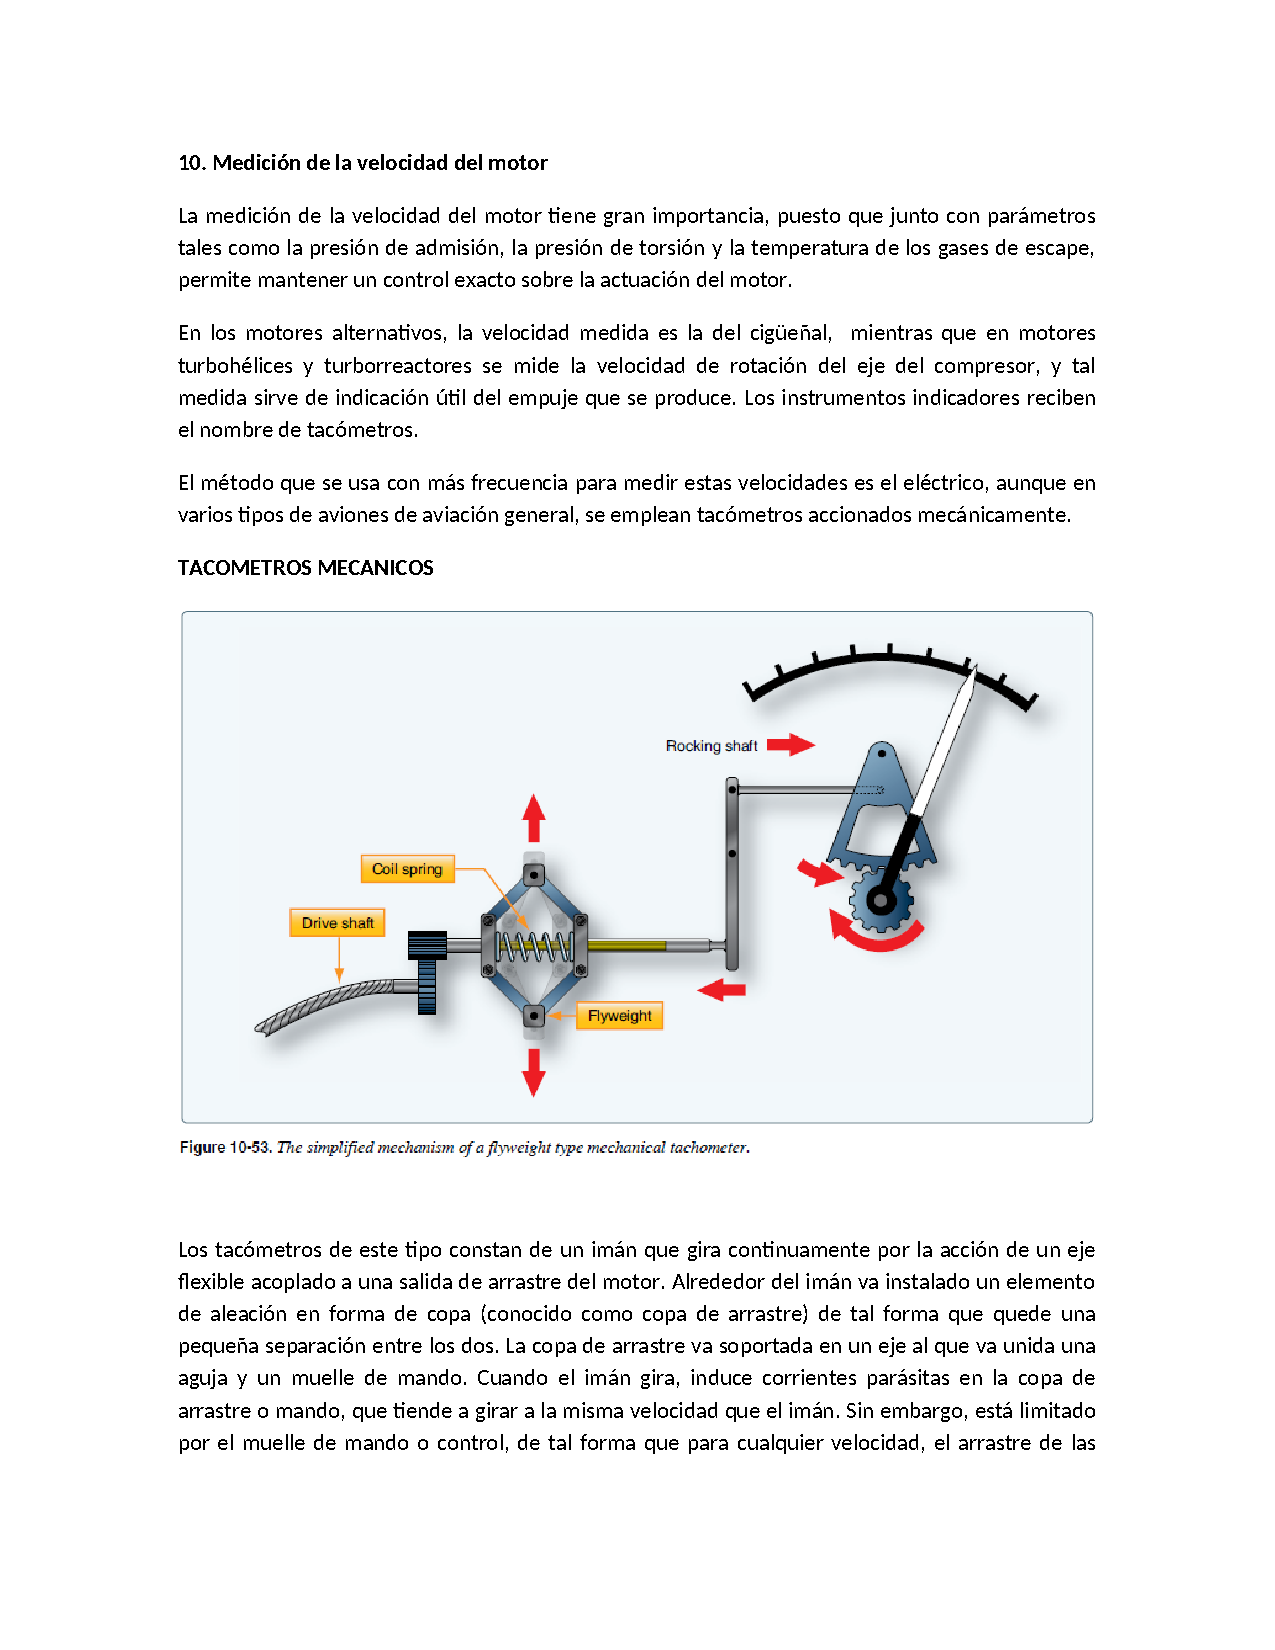
\includepdf[pages=-, fitpaper=false, scale=1.0, %landscape=true,
  offset = 0 -20,
  pagecommand={\thispagestyle{fancy}}]
{03.instrumentos.motores/Taquimetros.pdf}

\section{Flujómetros, diferentes tipos, totalizadores}
\label{sec:U03.02.flujometros}

  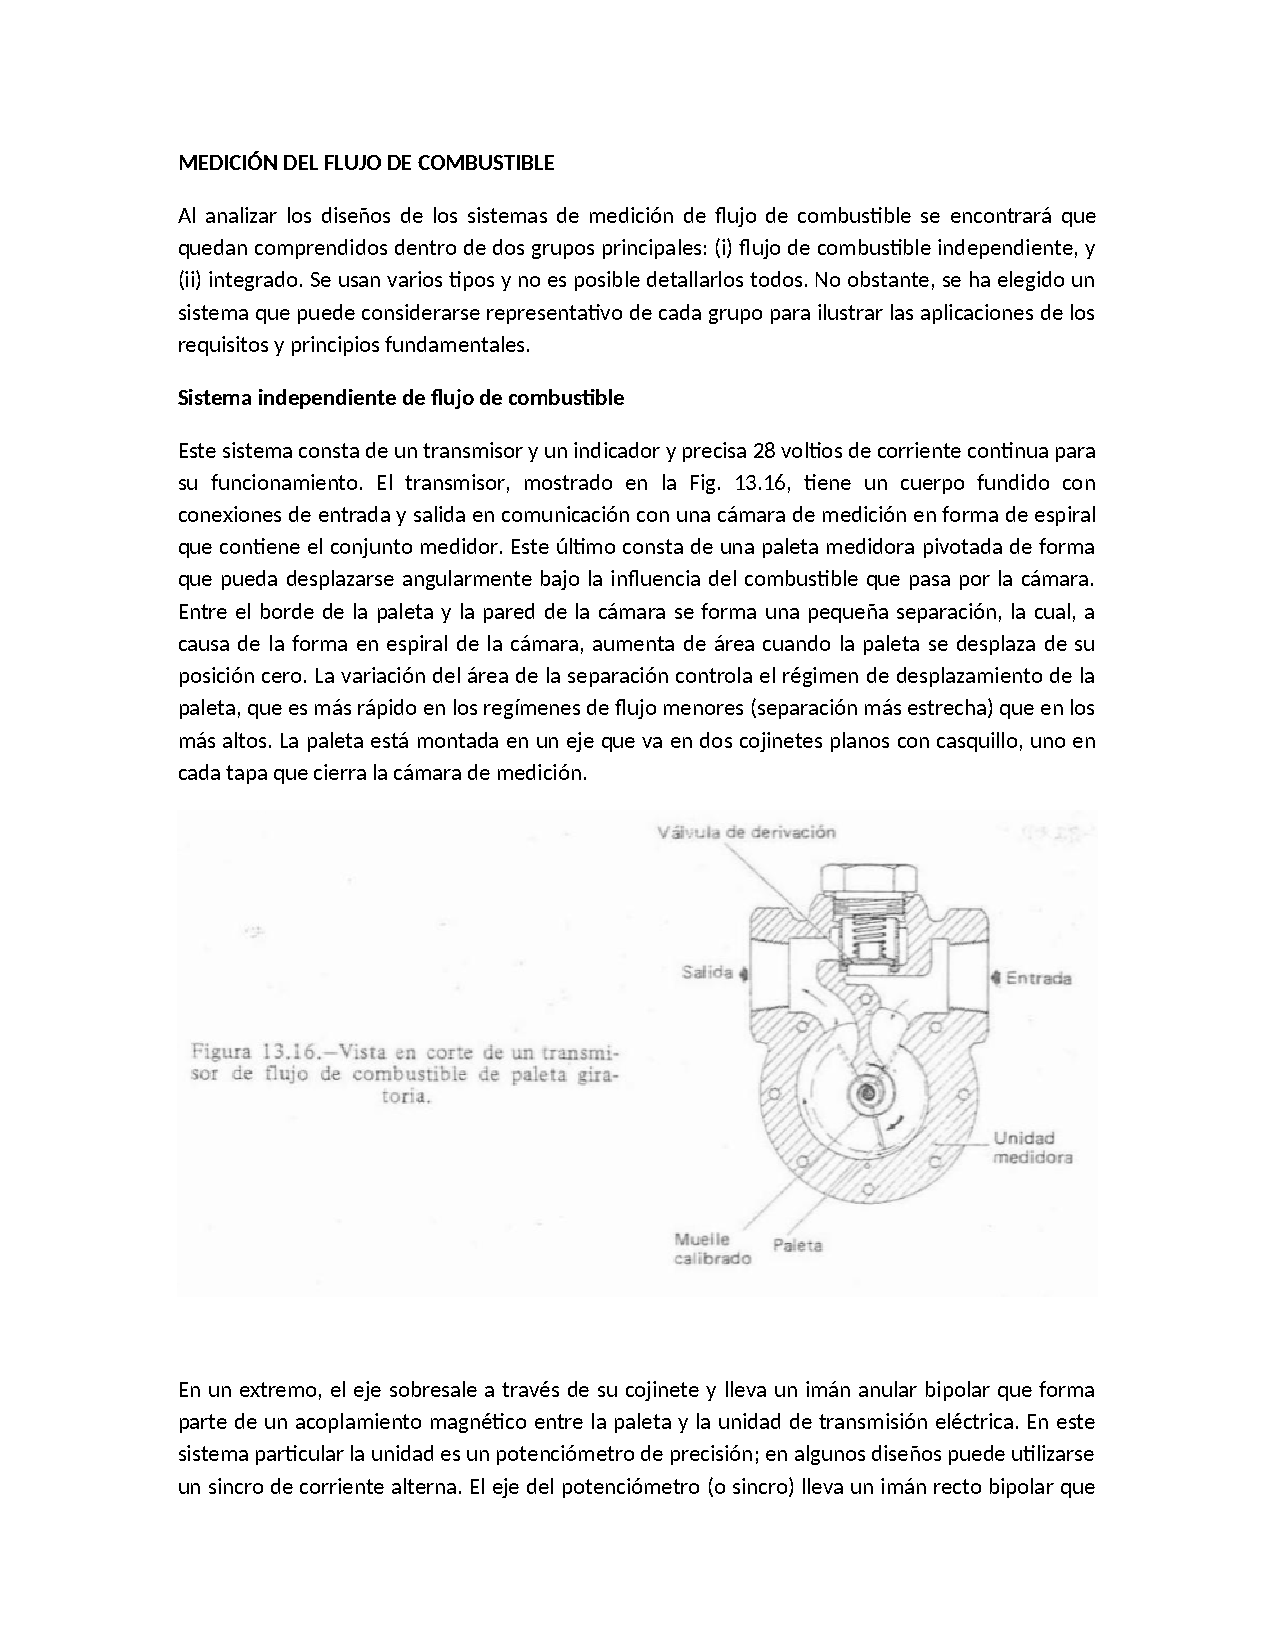
\includepdf[pages=-, fitpaper=false, scale=1.0, %landscape=true,
  offset = 0 -20,
  pagecommand={\thispagestyle{fancy}}]
{03.instrumentos.motores/MedicionDelFlujoDeCombustible.pdf}

% \section{Indicadores de empuje, indicadores de torque}
% \label{sec:U03.03.indicadores.empuje}

\section{Termocuplas. Medición de la temperatura en motores}
\label{sec:U03.termocuplas}


  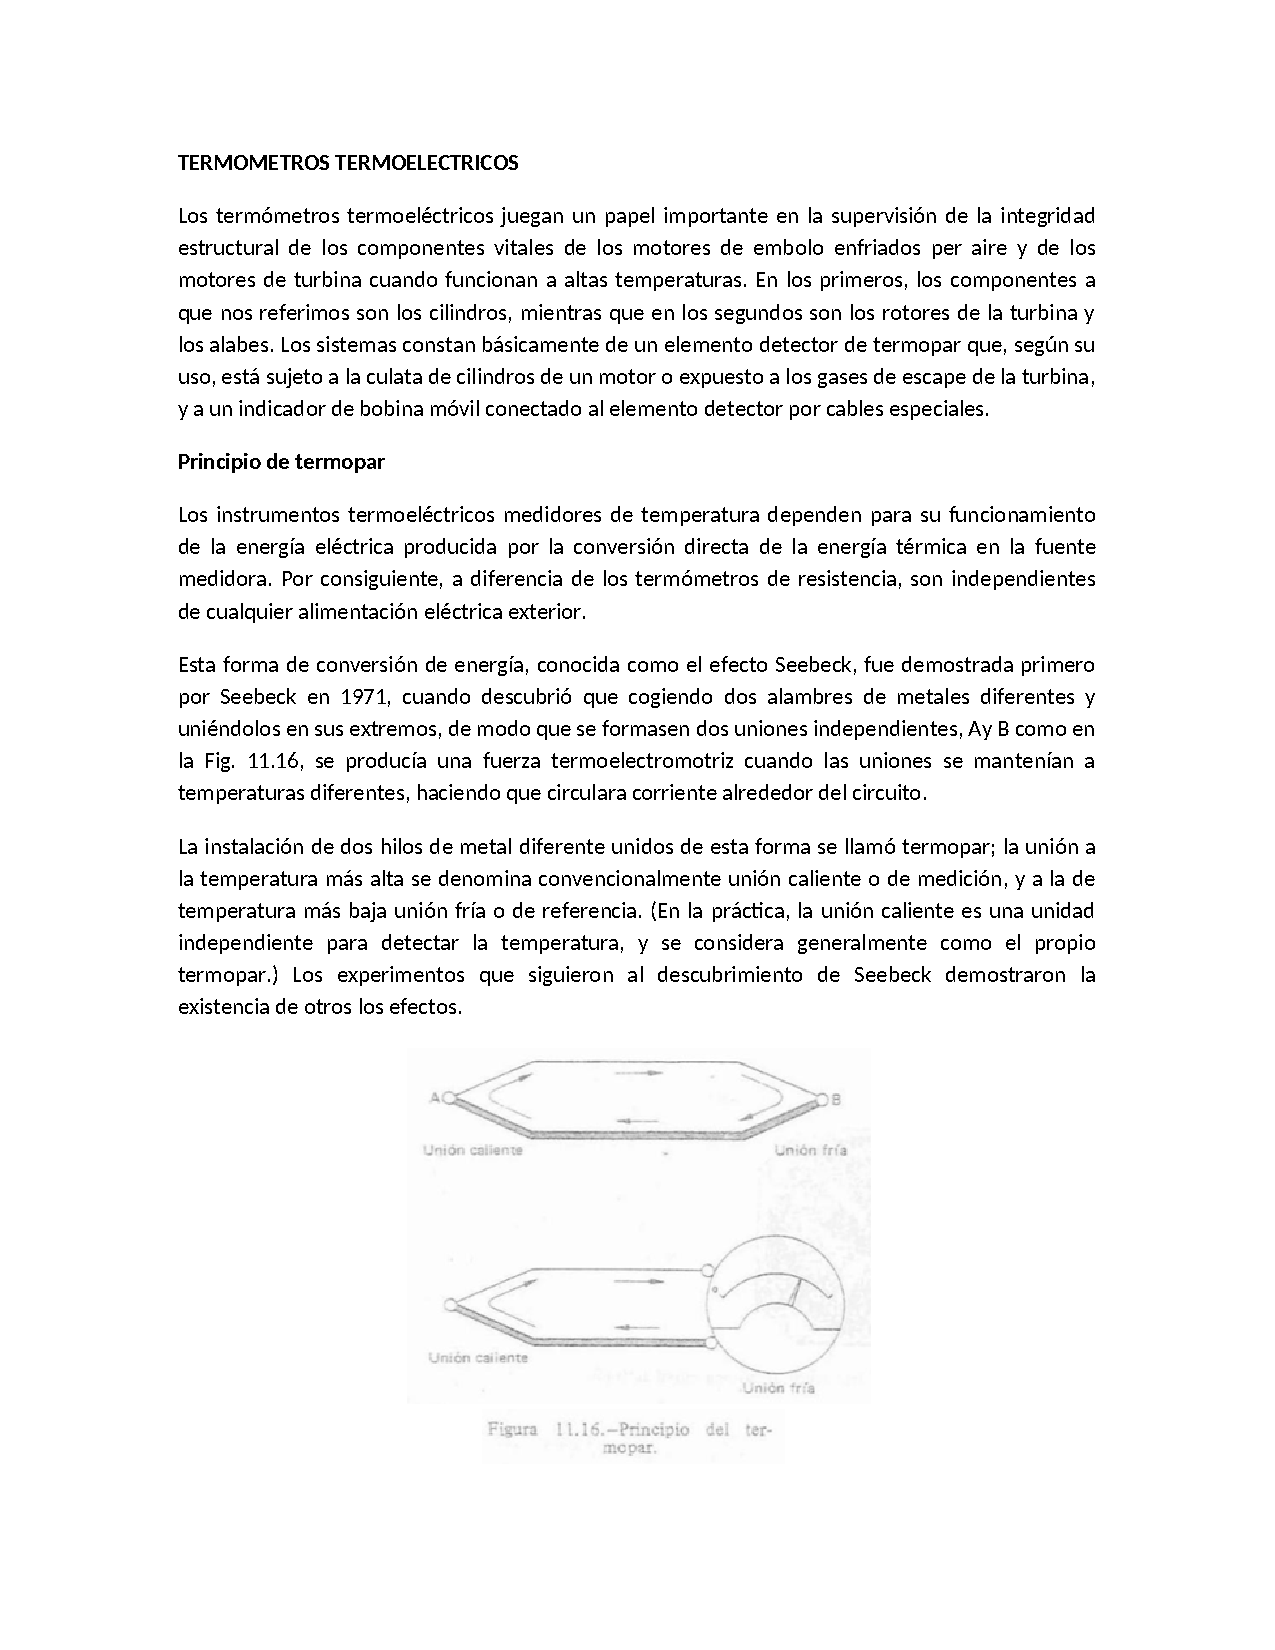
\includepdf[pages=-, fitpaper=false, scale=1.0, %landscape=true,
  offset = 0 -20,
  pagecommand={\thispagestyle{fancy}}]
{03.instrumentos.motores/MedicionDeTemperaturaEnMotoresTermometrosTermoelectricos.pdf}